\documentclass[10pt,a4paper,twocolumn]{article}

\usepackage{graphicx}
\usepackage{hyperref}
\usepackage[usenames]{color}

\definecolor{LinkColour}{rgb}{0,0.08,1}

\definecolor{URLcolour}{rgb}{0.5,0.08,1}

\hypersetup{
  pdftitle={ULTRACAM reduction guide},
  pdfauthor={Tom Marsh, Warwick},
  pdfborder={0 0 1},
  colorlinks=true,
  linkcolor=LinkColour,
  urlcolor=URLcolour,
%  linkbordercolor={0.5 0.57 0.72},
}

\author{T.R. Marsh}

\title{A Guide to the Reduction of ULTRACAM data\\ Version 0.3}

\date{\today}

\newcommand{\starlink}{Starlink}

% path to documentation
%\hyperbaseurl{file:}
\newcommand{\main}{http://quetzel.csc.warwick.ac.uk/phsaap/software}
\newcommand{\ultracam}{\main/ultracam/html}
\newcommand{\warn}[1]{\textcolor{red}{\emph{#1}}}

\begin{document}

\maketitle

\begin{abstract}
This document is a manual on the reduction of high-speed 
CCD photometry taken with ULTRACAM. The aim is to give a coherent
picture not afforded by the individual program descriptions.
This is a very rough first draft; I hope in the future to add
some graphics.
\end{abstract}

\section{Introduction}

While it is possible to get near-publication quality reduced data 
directly at the telescope with ULTRACAM, the main purpose of the 
near real-time reduction is to monitor data quality and to help with
observing decsions. Therefore you may well want to re-reduce the data
yourself. This document is a guide as to how one goes about this.
Note that there are lots of detailed program descriptions avaliable,
and so this document does not try to repeat these, rather its purpose is
serve as a guide for the whole reduction process and is based upon experience
of having used ULTRACAM for a while.

If you view this with acroread or 'kpdf' then you should be able to
see the hyper-links in your browser.

\section{Getting the software}

If you are going down the reduction route, you will need to install some software.
Please look at the \href{\main/index.html}{software web pages} for details
of how to do this. Let me know of problems that you encounter.

\section{Getting the data}

At some point we hope to make an automated database where you can pick
the files that you need. Until this point I'm afraid that it is a
matter of asking us for your data, and response is by no means
immediate. At Warwick I have much of the data on-line and can transfer
it to a web server for download and I hope to streamline this with time.

ULTRACAM data comes in the form of raw data files of the form 'run034.dat' and
for each one a corresponding XML file, e.g. 'run034.xml'. Both files must exist
in order to be able to do anything with the data.

\section{Reduction}

\subsection{First steps -- getting oriented}

Once you have the data the first thing is to see if you can plot some of it. 
fire up the software and try out the command
\href{\ultracam/rtplot.html}{rtplot}. You may need to point it at the right
source of data the first time you use it; look at the help. If it hangs,
ctrl-C, and then re-run specifying ``prompt'' on the command line. It is
probably looking for a non-existent server; you will want the ``local'' option.

Having done this to a few files, you might want to
\href{\ultracam/grab.html}{grab} a few files which you can then look at in more
detail with \href{\ultracam/plot.html}{plot} or
\href{\ultracam/cplot.html}{cplot}. The files are stored as files
with the extension '.ucm'. For instance you might end up with 'run034\_001.ucm',
'run034\_002.ucm' etc. Each of these contains all three CCDs plus some header
info. Try the program \href{\ultracam/uinfo.html}{uinfo} to get a little basic
data on a ucm file. The image display facilities in the pipeline software are
crude by comparison with 'ds9' or 'gaia'; it has not been my intent to replicate
such programs. If you want to use them then you should convert the files to
FITS which can do using \href{\ultracam/ucm2fits.html}{ucm2fits} for ucm files,
or more directly using \href{\ultracam/grab2fits.html}{grab2fits}. 

I now go through the reduction steps in the order in which you should approach
them. If you want a quick look you could at this point jump to the section
on apertures (section~\ref{sec:apertures}).

\subsection{Making bias frames}

Almost the first thing you should do is to create a mean bias
frame. With the two readouts/CCD of ULTRACAM the different bias levels
can make it hard to view images easily, so you will typically want to
remove the bias level fairly early on. Some frequently used commands, 
such as \href{\ultracam/rtplot.html}{rtplot} allow you to do so on the fly,
but you still need to supply a bias frame. Find a bias run, check the
comments to see that things were OK and then
\href{\ultracam/grab.html}{grab} the entire run. Make a list
containing all the names of the resulting ucm files (e.g. 'ls
run034*.ucm > bias.lis') and apply the program
\href{\ultracam/combine.html}{combine}. In the case of biases, it is much
better to use the
clipped mean method of combination rather than the median which
suffers from digitisation noise. You should use the 'bias' adjustment
to allow for variable bias levels. Note that you should select a bias
that matches your data pretty much in terms of setup, in particular
you should use a bias of the same readout speed (hex code in the logs)
and binning factors. The readout speed is not currently checked, but
you will not be able to use a bias of conflicting binning factors in
the main program \href{\ultracam/reduce.html}{reduce} unless you
re-format manually before running it.

\warn{Warning:} ULTRACAM sometimes suffers from a problem in which the bias levels
are incorrect immediately after a power-on. See
section~\ref{prob:bias} for more details.

You may have to make separate bias frames for your flat-fields and your data. 
Look at \href{\ultracam/makebias.html}{makebias} for a single command to
create a bias from a run. This will save you from grabbing, combining and
deleting intermediate files.

\subsection{Making dark frames}

The ULTRACAM chips run at $-40\,$C and have non-negligible dark
current, especially for exposures longer than a few seconds. Although
the mean dark current is less than 1 count per second, there are
various 'hot pixels' which can be far higher than this. Look at
your data with \href{\ultracam/rtplot.html}{rtplot} and see if you can
see obvious hot pixels. If you can then you might want to make a dark
frame. To do so you need a dark run, preferably taken during the night
because it very difficult to guard against light leakage during the
day. Grab these to ucm files, kick out any with non-standard exposures
times (probably the very first and very likely the last one) and
average together with \href{\ultracam/combine.html}{combine}. You
should either use the 'bias' or 'ignore' adjustment; I don't think it
should matter which.

Once you made the dark frame \warn{subtract the bias frame from it} otherwise
it will not work properly during reduction.

\subsection{Making flat fields}

ULTRACAM flats are typically taken as a long sequence at the start and end of
the night. The small deadtime of ULTRACAM is of great advantage and means that
we do not bother changing the exposure time as a rule. Typically the flats start
or end saturated in 2 or 3 of the chips, with the u' CCD being the least
sensitive and therefore coming out or going into saturation last of all. One
wants to median these for cosmic rays but this cannot be done directly because
of the changing mean level. On the other hand simply taking the median after
dividing out the mean level overweights low signal flats. Thus the routine
\href{\ultracam/makeflat.html}{makeflat} has been developed which takes the
median of small groups of normalised flats of similar mean level (prior to
normalisation) and then adds the results together with appropriate weights.
It also knows how to ignore saturated and 'peppered' (see below) flats.

\href{\ultracam/makeflat.html}{makeflat} works on lists of ucm files. 
\warn{You must subtract the bias before using it.} If you have a dark frame,
you should subtract it before running \href{\ultracam/makeflat.html}{makeflat} 
using \href{\ultracam/dsub.html}{dsub} which scales by the ratio of 
exposure times. For most pixels this should hardly matter, but there is no
reason not to try to correct hot pixels properly if possible.

\warn{Beware the last frame of a run!} Typically sky flats are terminated by
stopping the run in the middle of an exposure so the last exposure is
not to be relied upon. I always delete it after I have downloaded a run using 
\href{\ultracam/grab.html}{grab}. It only does not matter for bias frames.

Finally you should be aware of the \warn{peppering problem}
(section~\ref{prob:peppering}). This limits the frames that you can
use reliably to well below the normal 65535 saturation level. The script
\href{\ultracam/grms.html}{grms} has been created to make it easier to spot
peppering. It only does not matter for bias frames.

Be very careful with flat fields: if there are stars, they can leave traces if
you don't median them out sufficiently so experiment with varying the group
size if you have problems. \warnn{Always} look at the result!

\subsection{Making bad pixel frames}

 --- to be done --- not usually too important; mainly a data quality control
exercise.

\subsection{Setting up apertures}

\label{sec:apertures}

The software is not clever about apertures. You have to tell it where
each star that you want to reduce is. This has the advantage that it
is possible to cope with cases where a star disappears from view completely
-- you can still get an extracted count rate for what it is worth. Once you
have set them up at the start, the apertures are adjusted automatically frame by
frame you may be relieved to hear.

First of all you need to make an average frame of your target field. Use
\href{\ultracam/grab.html}{grab} to get a few suitable frames,
\href{\ultracam/combine.html}{combine} to average them, and subtract the bias.
No need to flat-field, unless you are trying for really accurate positions which
you expect to keep fixed in some way.

You then run \href{\ultracam/setaper.html}{setaper} on each CCD of the image.
This gives you options to link a faint star to a brighter reference stars and
so on. You may want to set a clean, isolated, bright star as a 'reference' in
any case is you are likely to want to measure the seeing or use apertures with
sizes that scale with the seeing. There are also options to mask stars that
might contaminate the sky apertures. See \href{\ultracam/setaper.html}{setaper}
for details.

The program writes an ASCII file which can be edited by hand as well, although
the format is fairly specific. Sometimes you may find that from one
night to the next that your target has drifted so far that it does not
get picked up. This can even happen during a night as differential
refraction moves the u' image relative to the others. If this is the
case, you can either relax the constraints in the reduction file (see
next) or you can apply \href{\ultracam/setaper.html}{setper} again to
re-centre the apertures.

\subsection{Reducing your data}

You are now almost ready to \href{\ultracam/reduce.html}{reduce} your
data.  You need only set up a data file to specify the reduction that
you want. This consists of an \href{\ultracam/reduce.red}{ASCII file}
with many options, for instance the names of the calibration files,
the method of extraction to use (optimal or normal), whether to vary
the aperture radii or hold them fixed, etc. If you have several runs,
I would strongly advise picking a 'typical' one first and adjusting
the parameters for it before running on all of the others. The program
\href{\ultracam/plot.html}{plot} which can b e set up to run through a
list of files may be useful here. (It is especially useful if you are
reducing 'foreign' format data consisting of a stack of CCD frames
where you want to check that they are all actually on the same
target). It is in particular tricky to pick
the optimal aperture scale if your using variable aperture radii.  In
Tim Naylor's optimal photometry paper, he recommends an aperture
radius of about 1.5 times the FWHM seeing. I find this to be OK for
faint targets, but it can be an underestimate for bright ones. This
can mean that one should use ratios or order 1.8 for the red and green
CCDs versus 1.5 for the ultraviolet. Use the multiple aperture radius
option together with the \href{\ultracam/splitr.html}{splitr} script
to reduce with many scale factors quickly.

Once you have the \href{\ultracam/reduce.red}{ASCII file} ready, then run it
using \href{\ultracam/reduce.html}{reduce}. The result is a large ASCII file
with many columns but it is self-documenting. Use your favourite program to
read the columns. You are on your own from this point; I am developing a program
to help but it is in a rather primitive state.

\subsubsection{Rebinning/cropping}

Because of time considerations we tend to take some calibration frames
unbinned, in particular flat-fields and darks. Bias frames on the
other hand must be taken with the correct binning. Given an unbinned
full-frame dark one can then match any binned and windowed setup by
appropriately binning it. This almost works for flats as well except
that one should divide them by the product of the binning factors to
ensure a mean level of one at the end;
\href{\ultracam/reduce.html}{reduce} 
now does this for you, but issues
warnings about it.

\section{Problems}

During the development of ULTRACAM several problems have been found and fixed,
affecting the data in various ways. I will describe these below; they
are summarised in Table~\ref{tab:glitches}.
\begin{table*}
\begin{tabular}{llp{3in}}
Problem & Dates affected & Comment \\
\hline
Midnight bug   & All                  & Software fix solves it completely.\\
Binning No.\ 1 & May 2002 -- Aug 2004 & Affects any binned data; flux
lost unrecoverably\\
Binning No.\ 2 & All?        & Pixel registration off in X by XBIN-1. 
Software fix available; needs to be settled for sure.\\
Peppering      & All                  & Up/down pattern seen if count
levels are high. A function of the 
vertical clocking time and particularly apparent on first night of
all, 16 May 2002 before we lengthened it. Solution: keep count levels low enough.\\
Bias level problems  & All & Sometimes the bias levels, particularly of the
red CCD can be quite different to normal and along with this extra
noise seems to be present. Solution: a restart always seems to fix it,
but you have to be on your toes to spot it. There are parameters in
\href{\ultracam/rtplot.html}{rtplot} to help.\\ 
\hline
\end{tabular}
\caption{Summary of ULTRACAM glitches\label{tab:glitches}}
\end{table*}
For some other problems that you may encounter during reduction, look at the
\href{\ultracam/FAQ.html}{FAQ}. 

\subsection{Midnight bug}
GPS time stamps are read every 10 seconds. For 10 seconds around midnight this
sometimes causes a problem where the times are off by an entire day. There is a
software fix for this which seems reliable, so it should not cause a problem.
You will occasionally see a warning however as midnight (UT) is passed.

\subsection{Binning problem No.\ 1}
This is the worst problem of all and is one that cannot be fixed. All runs 2002 to 2004
inclusive were affected by it. It was only spotted during the August 2004 run
and subsequently fixed. The problem occurred when binning in X. As a result of
inappropriate clears, this caused XBIN-1 out of XBIN pixels to be thrown away
losing large amounts of flux and potentially affecting photometric reliability.

Apart from the loss of flux, this also affects the practice of binning unbinned
calibration frames up to match binned frames. This must be done using 
\href{\ultracam/bcrop.cc}{bcrop} and you must \warn{not} 'coerce' the
calibration frames when running reduce as it will not do so correctly. Instead
you should make calibration frames that match your format using
\href{\ultracam/bcrop.cc}{bcrop}.

\subsection{Binning problem No.\ 2}
This is a new one as of January 2006 (discovery). It is possibly a
result of the fix for the first binning problem and therefore only
affects runs from 2005 onwards, but I am not sure. It may affect all
data binned in X. What seems to happen is that when binning the pixels
are mis-registered. e.g. in terms of unbinned pixels, pixels 1 to 3 of
a xbin=2 binned full-frame format represent pixels 0 and 1, 2 and 3, 4
and 5. Pixel '0' should not exist and so the outermost pixels on both
sides of the frame are in fact rubbish. This causes problems when
using calibration frames taken unbinned unless the mis-registration is
allowed for.  Tests in March 2006 reveal that the problem generalises
in the following way: basically one must shift the windows away from
the centre of the CCDs by XBIN-1 pixels from what one would
anticipate.

\emph{Still to determine: does this apply to data taken before May
  2005?}

\subsubsection{Peppering}
\label{prob:peppering}
At high counts levels, but well below saturation, the ULTRACAM chips show a
pattern in which neighbouring pixels are high and low.  This looks a bit like
pepper in the centres of the chips at high count levels, and thus we call it
peppering. This peppering occurs short of 30,000 counts in the green and
ultra-violet chips and at about 50,000 in the red CCD. \warn{You should set the
levels in \href{\ultracam/makeflat.html}{makeflat} to avoid frames affected by
peppering!} Use \href{\ultracam/rtplot.html}{rtplot} to find out the levels.
The maximum values I use are 48000, 30000 and 26000 for the red, green and
ultraviolet CCDs respectively (numbers 1, 2 and 3 as far as the software is
concerned). Peppering looks terrible when you first see it, but it really 
switches off as long as one is below the threshold levels.

\subsubsection{Bias level problems}
\label{prob:bias}

ULTRACAM sometimes suffers from a problem in which the bias levels are
incorrect immediately after a power-on. At the same time, increased
noise is present. The problem is worst for the red CCD.  Be careful to
check that such frames match other ones. Only use biases affected by
odd bias levels if your data suffer from the same problem. The program
\href{\ultracam/rtplot.html}{rtplot} can be set to provide a warning
of possible problems with the bias level. It may still be worth
reducing such data as it often far from useless.

\appendix

\section{ULTRACAM timing}

\subsection{Introduction}

This appendix details how the ULTRACAM times are generated. This is
complicated by various bugs and changes over the years. First I
summarise how the times come about. 

Each frame comes with 24 bytes of timing information generated at a
specific part of the readout/exposure cycle which I discuss in detail
below. The times are generated as follows. Every 10 seconds the GPS is
polled for the latest time, and at the same time the timing card is
polled. Then when the time for a frame is needed, the timing card is
queried again and the difference between this value and the value
recorded at the the time of the GPS poll is used to come up with the
final timestamp that is attached to the data.

In the ULTRACAM pipeline the times are handled by the routine
\emph{read\_header.cc}. The aim is to generate a UT date and time
corresponding to the \emph{middle of each exposure}. The GPS
timestamp gives the number of seconds from the start of the week
(defined as midnight on the saturday/sunday transition) and the number
of nanoseconds in addition to this (i.e this lies in the range 0 to
999999999. It also gives a date. So the standard is to add whatever
seconds are left after removal of integer*86400 + nanoseconds/1e9 to
the date.

This is by no means all there is to do, because to correct to the
middle of the exposure then depends upon the readout mode. However
before getting to this point one has to translate the GPS timestamp
into a time, and here there are several variants owing to changes. I
now detail these.

\subsection{Special cases}

Here I detail all the special cases that have affected the timestamps.

\subsubsection{May 2002 run}

This was the first ULTRACAM run of all and unsurprisingly things were
not honed to perfection. The timestamps of this run had no date
information, and so the known start of week date (12 May 2002) is used
to offset from. There was moreover an error where some times jumped
back by 10 seconds (related to the GPS polling time). This is
corrected by seeing if a time is less than an earlier one. I don't
think this ever causes problems, but could do if it is the first frame
of all that is wrong. Luckily it is usually a fairly short lived
problem.

In addition, the first night of the May 2002 run had a short vertical
clock time that caused the nasty "peppering" effect on the CCD. The
parameter VCLOCK\_FRAME is set specially for this night. The
vclock\_frame was not stored in the XML in this run so known numbers
are used for all nights of this run (these are needed for the
correaction to the mid-point of the exposures).

\subsubsection{September 2002 run}

This was the second ULTRACAM run. From the second night of this run we
had date information. Unfortunately, the year was not always right and
so special code fixes this to 2002. On top of this, day numbers were
only correct to within 1 day, changing incorrectly near midnight. They
are therefore used to identify the week in question, and then the
number of seconds is used as in the May 2002 case. 

\subsubsection{No GPS mode}

Without the GPS one can still get relative times from the
computer. These are indicated by the number of satellites = -1. The
date is then set to an arbitrary 1 Jan 2000 (i.e. before ULTRACAM
started) and the number of seconds etc is added to it. The number of
seconds however is now from the start of loading the software and
therefore does not mean anything in absolute terms.

\subsubsection{Midnight bug}

I discussed the midnight bug earlier. To repeat, frames taken near UT
midnight can suffer from the following problem: the number of seconds
indicates that the date has changed, but the date itself has yet to
update. This perhaps reflects some sort of offset in the polling time
for the date versus the time. I now correct for these by comparing the
say of the week implied by the number of seconds with the day of the
week implied by the GPS date. If these differ, 1 day is added to the
GPS date. A warning is issued; the correction seems 100\% reliable.


\subsection{Correcting the times for the readout mode}

Once the GPS time has been processed as above, it needs to be corrected to the mid-exposure
time. This is a function of the readout mode. In some cases one must have read the time of the
frame before to make this correction, or even several frames before (drift mode). If this is not possible
(e.g. first frame or frames) the time will be flagged as being not OK (NOK). 
\emph{NB.} If nsat=-1, the time may still be flagged as "OK" which it is as far as the
exposure correction, but not otherwise.

The timestamps are taken at particular parts of the cycle. The exact
point changed with a change from the old 50MHz to the new 250MHz
timing board that happened in July 2003. In the 50MHz system
timestamps were taken when a special timestamp bit was cleared. In the
250MHz system (current), timestamps are taken when this bit is
set. This change was not documented and we did not realise it for
sometime (until late 2004). It caused timestamps to be taken at
different points. This leads to different corrections according to the
board in place as well as the readout mode. To confuse matters
further, the sense of when the timestamps were taken with the 250MHz
board was reversed when the error was realised. This fix dates from
around Jan 2005 and returned things to pre-July 2003 days.

I now go through the event sequences for the differing modes. I will
use the terms 'standard' and 'non-standard' to denote the times when 
things operated as documented versus when they did not. i.e. ``standard'' 
covers before July 2003 and after January 2005, while ``non-standard''
covers the inter-regnum.

\subsubsection{Full-frame + clear, full-frame + overscan and 2-window + clear modes}

These modes have clears in them to allow accurate exposure lengths and
to avoid saturation on bright targets. They are standardly used for
standard stars and sky flats. The order of events in these modes is as follows:
\begin{enumerate}

\item Set timestamp bit. 

\item Clear the CCD.

\item Clear the timestamp bit. Standard timestamp.

\item Expose the CCD

\item Frame transfer

\item Read CCD

\item Set the timestamp bit. Non-standard timestamp.

\item Go back to stage 2 unless the run is stopped.

\end{enumerate}
\begin{figure*}
\hspace*{\fill}
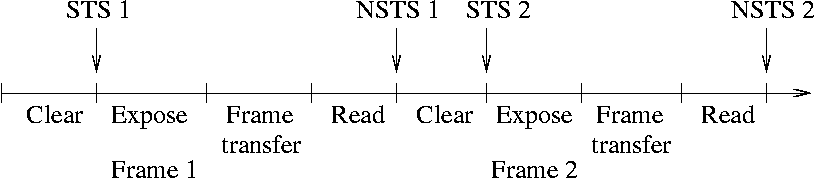
\includegraphics[width=0.8\textwidth]{clear_modes}
\hspace*{\fill}

\caption{The sequence of events in the various ``clear'' modes. Note
  that in this case ``Expose'' is the only time during which photons
  are accumulated. ``STS'' indicates a standard timestamp, ``NSTS'' a
  non-standard timestamp.}
\label{fig:clear_modes}
\end{figure*}
These events are displayed graphically in
Fig.~\ref{fig:clear_modes}. In interpreting this diagram it is
important to realise that timestamp $N$ is always paired with frame
$N$, even when it is readout afterwards because the frames and
timestamps are buffered and then written to disk together. 

Non-standard timestamps are generated when the timestamp bit goes from
clear to set. This could happen at the start if the bit started clear.
However, I believe that this is never the case from looking at many runs and
also from a communication from Dave Atkinson. This is lucky since
otherwise we could have had one frame offsets in the timestamps.

In standard mode the time at the mid-point of the $n$-th frame
$(t_m)_n$ is simply given by
\begin{equation}
(t_m)_n = (t_s)_n + \frac{\Delta}{2},
\end{equation}
where $(t_s)_n$ is the time of the timestamp associated with the
$n$-th frame and $\Delta$ is the length of the exposure, aka the 
``exposure delay'', and in this case is the true on-target time.

Things are trickier in non-standard mode. If one looks at the order of
events in Fig.~\ref{fig:clear_modes}, one sees that the non-standard
timestamp of any frame is taken after it has been frame transferred
and read out, so that one would have to subtract an estimate of these
quantities to get to the mid-exposure. This cannot be done very
accurately. The best thing is to forward track from the previous
timestamp (possible for all frames except the first) by adding the 
clear time, e.g.
\begin{equation}
(t_m)_n = (t_s)_{n-1} + t_c + \frac{\Delta}{2},
\end{equation} 
where $t_c$ is the time taken to clear the CCDs. This is estimated using
\begin{equation}
t_c = (1033 + 1027) t_{vc},
\end{equation} 
where $t_{vc}$ is the time taken to vertically clock a frame by 1
pixel, a clear requiring clocking of the entire image and storage areas.
$\Delta$ is still the length of the exposure. If the previous
timestamp is not present, then one must fall back on
\begin{equation}
(t_m)_n = (t_s)_n - t_{ft} - t_r - \frac{\Delta}{2},
\end{equation} 
where $t_r$ is the readout time and $t_{ft}$ is the frame transfer
time. I am unclear about the reliability of either, but in the end I
decided to mark the times returned by the first equation as reliable
and the times returned by the second as unreliable as the readout time
is difficult to estimate reliably.

\subsubsection{Full-frame no-clear and windowed modes}

These are the standard science modes. The order of events is as follows:
\begin{enumerate}

\item Set timestamp bit. 

\item Clear the CCD.

\item Expose the CCD

\item Frame transfer. 

\item Clear the timestamp bit. Standard timestamp.

\item Read CCD

\item Set the timestamp bit. Non-standard timestamp.

\item Go back to stage 3 unless the run is stopped.

\end{enumerate}
\begin{figure*}
\hspace*{\fill}
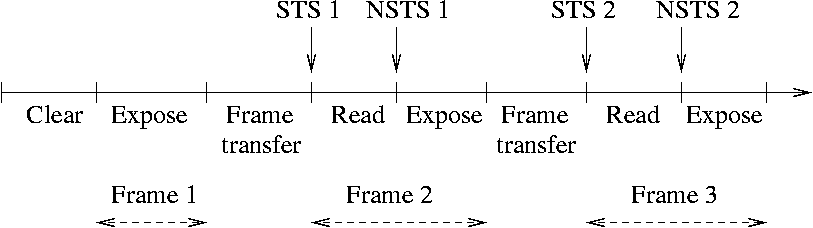
\includegraphics[width=0.8\textwidth]{window_modes}
\hspace*{\fill}

\caption{The sequence of events in the full-frame clear, windowed and
driftscan modes. Photons are accumulated during both the ``Expose''
and ``Read'' sections. Note that the first frame accumulates photons
for a shorter time than the rest.}
\label{fig:window_modes}
\end{figure*}
These events are displayed graphically in Fig.~\ref{fig:window_modes}

In standard windowed modes, photons start accumulating immediately
after the timestamp of the \emph{previous} frame is taken and while
that frame is being read out. They do so for the length of time it takes to read the previous frame
plus the exposure delay. Thus one can derive the time of mid-exposure
by adding half of the sum of the read time plus exposure delay to the
previous timestamp. The following formula does just this:
\begin{equation}
(t_m)_n = (t_s)_{n-1} + \frac{1}{2}\left( (t_s)_{n} - (t_s)_{n-1} -  t_{ft} \right).
\end{equation} 
where $t_{ft}$ is the frame transfer time which must be estimated.
Thus one must have read the timestamp immediately preceding a frame as
well as its own to derive the mid-exposure time in standard windowed
mode. The quantity in brackets is the on-target exposure time 
for exposure $n$:
\begin{equation}
(t_e)_n = (t_s)_{n} - (t_s)_{n-1} -  t_{ft},
\end{equation}
which is used to get the count rates.

In non-standard mode the timestamp is delayed until after the read. 
The question is, does this timestamp therefore get associated with
the data of the \emph{following} read, or are the data read out
buffered so that the timestamp can be attached to them? If the former,
what timestamp does the very frame of all get? This question is
important because it means a shift by one frame of which timestamp
goes with which frame. I believe that the second alternative is true,
i.e. even though the timestamp is taken after the data are read, it
still is written to disk with them. This is a conclusion based upon
looking at the timestamps of non-standard mode drift exposures.
This is how I have drawn it in Fig.~\ref{fig:window_modes}.
 
We again  need to adjust to the centre of the exposure which now
requires adding $(\Delta - t_r)/2$ where $t_r$ is the length of the
read immediatly preceding the (non-standard) timestamp taken
\emph{before} the current timestamp. This can be estimated using
\begin{equation}
t_r = (t_s)_{n-1} - (t_s)_{n-2} -  t_{ft}  - \Delta,
\end{equation}
and so 
\begin{equation}
(t_m)_n = (t_s)_{n-1} + \Delta - \frac{1}{2}\left( (t_s)_{n-1} - (t_s)_{n-2} -
        t_{ft} \right).
\end{equation} 
Similarly the on-target time is given by
\begin{equation}
(t_e)_n = (t_s)_{n-1} - (t_s)_{n-2} -  t_{ft}.
\end{equation}
Thus in non-standard mode one must keep the two timestamps preceding
the current one to get the mid-exposure of a given frame.

\subsubsection{Drift mode}

The sequence of events in drift mode is identical to that in windowed
mode except that the frame transfer stage is not a complete shift but
just moves the windows into the storage area. The series of windows in
the storage eventually gets read out once enough of them have been
moved in. The advantage of this is that the shift from image to
storage is relatively small. An additional complication is that every
so often an extra ``pipeshift'' is needed to bring the frames on the
storage area up to where they can be read out. This is because the
windows do not divide into the available storage exactly. The
pipeshift adds to the read times of the cycle in the previous
section. Although this all sounds complicated it is not if one
realises that normal windowed mode is essentially drift mode with only
1 window in the storage area. In drift mode there are, let us say, $N$
windows in the storage area which simply shifts the relation between
timestamps and frames by $N-1$. Thus the equations of the previous
section become
\begin{equation}
(t_m)_n = (t_s)_{n-N} + \frac{1}{2}\left( (t_s)_{n-N+1} - (t_s)_{n-N} -  t_{ft} \right),
\end{equation}
for standard mode and
\begin{equation}
(t_m)_n = (t_s)_{n-N} + \Delta - \frac{1}{2}\left( (t_s)_{n-N} -
  (t_s)_{n-N-1} - t_{ft} \right)
\end{equation} 
for non-standard mode. Here the frame transfer time $t_{ft}$ must be estimated
differently than for the windowed mode because only a small shift onto the
storage area is needed. Application of these relations require storage of
timestamps read out several frames ahead of the one of interest.
This is done with a data structure that one can 'pop' and 'push' 
elements onto inside \emph{read\_header.cc}. The first $N-1$ frames read
out are junk data which have only ever been in the storage area. The
$N$-th frame read is the first to have any proper photons, but its 
time cannot be determined because there is no $(t_s)_{n-N}$ for $n =
N$. Thus the first usable frame is therefore frame $N+1$.

The on-target exposure times are similarly shifted:
\begin{equation}
(t_e)_n = (t_s)_{n-N+1} - (t_s)_{n-N} -  t_{ft},
\end{equation}
and
\begin{equation}
(t_e)_n = (t_s)_{n-N} - (t_s)_{n-N-1} -  t_{ft}.
\end{equation}

\end{document}
